\input{free-speech-ott}

\renewcommand{\FSdrulename}[1]{\scriptsize \textsc{#1}}

\newcommand{\tvdash}[1]{\vdash^{#1}}
\newcommand{\arrowT}[5]{(#1 :^{#2} #3)^{#4} \to #5}
\newcommand{\rec}[3]{rec\ #1\ #2\ #3}
\newcommand{\recc}[3]{rec^{-}\ #1\ #3}

The requirement that every program must terminate can be relaxed by
first designing a very powerful programming language (PL), and then
carving out two fragments of programs. The first consists of all the
terminating programs called the logical fragment, and the second
consists of all programs, and this is called the programmatic
fragment. That is we have a picture that looks something like:
\begin{center}
  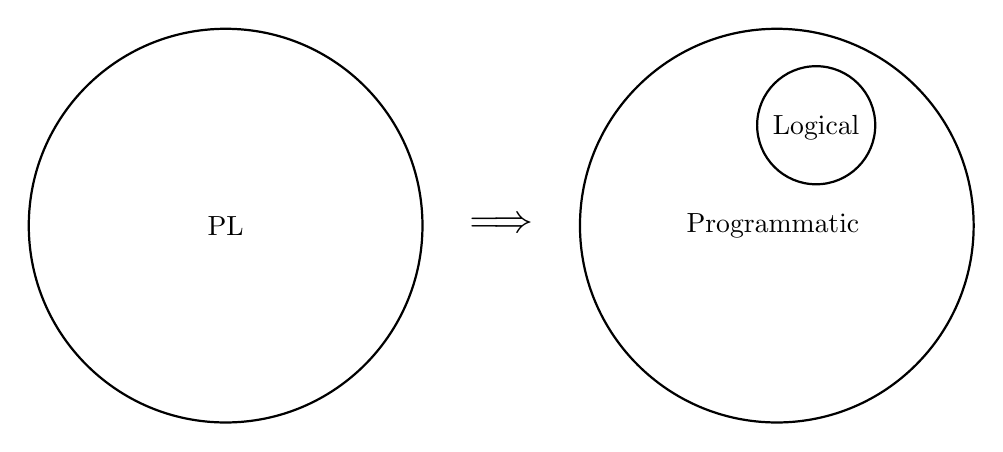
\begin{tikzpicture}[scale=2.5,cap=round,>=latex]
    % draw the unit circle
    \draw[thick] (0cm,0cm) circle(1cm);
    \draw (0cm,0cm) node {PL};
    \draw (1.4cm,0cm) node {\Large $\Longrightarrow$};
    \draw[thick] (2.8cm,0cm) circle(1cm);
    \draw (2.78cm,0cm) node {Programmatic};
    \draw[thick] (3cm,0.51cm) circle(0.3cm);
    \draw (3cm,0.5cm) node {Logical};
  \end{tikzpicture}
\end{center}
The logical fragment will then be considered the ``logical framework''
of the language, and this is where the programs are proofs and the
types are propositions, that is the logical fragment makes use of the
computational trinity (Chapter~\ref{chap:the_three_perspectives}).
Now the programmatic fragment is where all the usual programming will
take place, then one can use the logical fragment to verify properties
of the programs written in the programmatic fragment.  However, the
programming language will need some additional features to make this
all work.

Once the logical fragment has been identified three additional
features will need to be added.  The first feature is that types in
the logical fragment will need to be able to depend on programs from
the programmatic fragment, but this feature has to be designed so as
to prevent these programs from being applied to any arguments or this
would prevent the logical fragment from being logically consistent.
For an overview of logical consistency and how it can be proven see
Chapter~\ref{chap:metatheory_of_programming_languages}.  We call this
feature freedom of speech, because it intuitively states that logical
types and programs can talk about potentially non-terminating
programs, but they are never allowed to actually run them.

The second and third features are usability features.  The logical
fragment is purely specificational.  Its primary use is for the
verification of programs written in the programmatic fragment.
Furthermore, carrying around non-computationally interesting proofs is
expensive.  Thus, it is important to allow some specificational data
to be stripped away during compile time.  In addition, it is important
that the programmer be the one to decide which data is removed.  Now
logical programs are proofs, but they are also terminating programs,
and thus can be considered both logical programs and programmatic
programs.  The third and final feature is the ability to write
programs in the logical fragment and then move them into the
programmatic fragment.  This facilitates code reuse and provides a
means to write verified terminating programs.

In this chapter we introduce the design of a programming language that
contains all of these features, and some additional ones.  It is
called Freedom of Speech, because it is the first core
dependently-typed functional programming language with the freedom of
speech property.  The syntax and the CBV reduction relation is defined
in Figure~\ref{fig:FS-syn-red}.  
\begin{figure}
  \begin{center}
    \begin{tabular}{lll}
      Syntax:
      \vspace{10px} \\
      \begin{math}
        \arraycolsep=2pt\edef\arraystretch{1.2}
        \begin{array}{rllllllllllllllll}
          \text{(Classifiers)}  & [[th]] & ::= & [[L]]\,|\,[[C]]\\
          \text{(Stages)}       & [[ep]] & ::= & [[+]]\,|\,[[-]]\\
          \text{(Expressions)}  & [[e]]  & ::= & 
          [[Type]]\,|\,[[Nat]]\,|\,[[x]]\,|\,[[(x : th e1) ep -> e2]]\,|\,[[e1 = e2]]\,|\,
          [[S]]\,|\,[[Z]]\,|\,\\
          & & & [[\x.e]]\,|\,[[rec f x e]]\,|\,[[rec - f e]]\,|\,[[e1 e2]]\,|\,
                [[join]]\,|\,[[injdom]]\,|\,[[injran]]\,|\,\\
          & & & [[contra]]\,|\,[[abort]]\\
          \text{(Values)}       & [[v]] & ::= & 
          [[x]]\,|\,[[Type]]\,|\,[[Nat]]\,|\,[[(x : th v1) ep -> v2]]\,|\,
          [[e1 = e2]]\,|\,[[\x.e]]\,|\,\\
          & & & [[join]]\,|\,[[injdom]]\,|\,[[injran]]\,|\,[[rec f x v]]\,|\,[[rec - f v]]\\
          \text{(Evaluation Contexts)} & [[C]] & ::= & [[ [] ]]\,|\,[[( x : th C ) ep -> e2]]\,|\,[[( x : th e1 ) ep -> C]]\,|\,[[rec f x C]]\,|\,\\
          & & & [[rec - f C]]\,|\,[[e1 C]]\,|\,[[C v]]\\
          \text{(Typing Contexts)}     & [[G]] & ::= & [[.]]\,|\,[[x : th e]]\,|\,[[G1,G2]]\\        
        \end{array}
      \end{math}\\
      & \\
      CBV reduction:\\
      \small
      \begin{mathpar}
        \FSdruleCbvXXApp{}  \and
        \FSdruleCbvXXRec{}  \and
        \FSdruleRedXXCtxt{} \and
        \FSdruleRedXXAbort{} \and
        \FSdruleComputeJoin{}
      \end{mathpar}
    \end{tabular}
  \end{center}  
  \caption{Syntax and reduction rules for freedom of speech}
  \label{fig:FS-syn-red}
\end{figure}
The syntax is collapsed similarly to the Calculus of Constructions --
see Chapter~\ref{sec:the_calculus_of_constructions} for more about the
Calculus of Constructions. So we distinguish between types and terms
(programs) judgmentally.  Expressions and the typing judgment will
depend on two annotations.  The first is called the consistency
classifier and is denoted $[[th]]$ which can be one of $[[L]]$ or
$[[C]]$ where an expression tagged with the former is interpreted to
mean ``belonging to the logical fragment'' and the latter to mean
``belonging to the programmatic fragment.''  The second annotation is
denoted $[[ep]]$ which is called the stage annotation and can be
either $[[+]]$ or $[[-]]$ where the former means ``run time'' and the
latter means ``compile time.'' The consistency classifier essentially
is how we carve out the logical fragment from the programmatic
fragment, and the stage annotation implements the second feature above
where all programs marked as compile time will be erased before run
time.  We now give a brief overview of the syntax of Freedom of
Speech.

Expressions denoted $[[e]]$,$[[e_1]],\ldots,[[e_i]]$ consist of
$[[Type]]$ which is the type of all types, $[[Nat]]$ the type of
natural numbers, variables denoted $[[x]]$,$[[y]]$,$[[z]]$, $\ldots$,
dependent function types denoted $[[(x : th e1) ep -> e2]]$ -- note that
the programmer gets to decide whether an argument is ``logical'' or
``programmatic'' and ``run time'' or ``compile time'' -- next we have
equations denoted $[[e1 = e2]]$, the successor function and the
natural number zero denoted $[[S]]$ and $[[Z]]$ respectively,
$\lambda$-abstractions denoted $[[\x.e]]$, two recursors $[[rec f x
e]]$ and $[[rec - f e]]$ where $[[x]]$ is considered bound in $[[e]]$
in the former, application denoted $[[e1 e2]]$, three forms of proofs
of equations denoted $[[join]]$, $[[injdom]]$, and $[[injran]]$, where
the latter two are injectivity proofs and are discussed further below,
and finally we have two forms of contradictions one logical and one
programmatic denoted $[[contra]]$ and $[[abort]]$ respectively.

The CBV reduction relation is broken up into three different
judgments.  The first is denoted $[[e1 ~b> e2]]$ and defines standard
CBV $\beta$-reduction and consists of two rules
$\FSdrulename{CBV\_App}$ and $\FSdrulename{CBV\_Rec}$ where values are
defined in Figure~\ref{fig:FS-syn-red}.  We will see that the latter rule
can be used for both terminating and non-terminating recursion
depending on which fragment the recursor is typed in.  Note that there
are no congruence rules in the definition of the first judgment.  The
second judgment denoted $[[e1 ~> e2]]$ extends the first with
congruence rules, and a rule for aborting a contradictory computation.
This judgment consists of two rules $\FSdrulename{Red\_Ctxt}$ and
$\FSdrulename{Red\_Abort}$.  These two are defined in terms of
evaluation contexts which can be thought of as a means of specifying
where with in an expression computation can take place. The syntax of
evaluation contexts can be found in Figure~\ref{fig:FS-syn-red}.  This
defines a fragment of the syntax of expressions where exactly one well
formed subexpression has been replaced with a hole.  Holes are denoted
$[[ [] ]]$. Lets consider a few examples:
\begin{example}
  \label{ex:FS-WF-ECTX}
  The following are all well-formed contexts:
  \begin{center}
    $[[((\x.S x) []) ]]$, $[[ ([] Z)]]$, and $[[rec f x (rec g y [])]]$.
  \end{center}
  Now $(\lambda x.[[S]]\,[[ [] ]])\,[[Z]]$ and $[[ [] ]]\,[[ [] ]]$
  are not well-formed contexts.
\end{example}
\noindent
In addition to the syntax of evaluation contexts we also define an
operation that takes an evaluation context and an expression and
``plugs'' the expression into the hole of the context.  

\begin{definition}
  \label{def:FS-ectx-plug}
  Plugging an expression $[[e]]$ into an evaluation context $[[C]]$ is denoted $[[C[e] ]]$
  and is defined by recursion on the form of $[[C]]$ as follows:
  \begin{center}
    \begin{math}
      \begin{array}{rll}
        [[ [] [e] ]]                    & = & e\\
        [[(( x : th C ) ep -> e2)[e] ]] & = & [[( x : th C[e] ) ep -> e2]]\\
        [[(( x : th e1 ) ep -> C)[e] ]] & = & [[( x : th e1 ) ep -> (C[e]) ]]\\
        [[(rec f x C)[e] ]]             & = & [[rec f x (C[e]) ]]\\
        [[(rec - f C)[e] ]]             & = & [[rec - f (C[e]) ]]\\
        [[(e1 C)[e] ]]                  & = & [[e1 (C[e]) ]]\\
        [[(C v)[e] ]]                   & = & [[(C[e]) v]]\\
      \end{array}
    \end{math}
  \end{center}
\end{definition}
At this point one can easily see that the $\FSdrulename{Red\_Ctxt}$
and $\FSdrulename{Red\_Abort}$ are actually a family of congruence
rules parametric in the evaluation context $[[C]]$. Now the rule
$\FSdrulename{Red\_Ctxt}$ simply extended the CBV $\beta$-reduction to
evaluation contexts, while the rule $\FSdrulename{Red\_Abort}$ says
that if $[[abort]]$ appears anywhere in an evaluation context, then the
computation is aborted and concludes just $[[abort]]$.  Lets consider
an example using what we have introduced thus far before moving onto
the type system.

\begin{example}
  \label{ex:FS-syn-red-case}
  First, we define the booleans and boolean case analysis just as we did
  in system F (see Example~\ref{ex:F_terms} in
  Chapter~\ref{chap:the_history_of_type_theory}):
  \begin{center}
    \begin{math}
      \begin{array}{lll}
        \mathsf{Bool}  \defeq [[(x : C Type)+ -> (y : C x) + -> (z : C x)+ -> x]]\\
        \mathsf{True}  \defeq [[\x.\y.\z.y]]\\
        \mathsf{False} \defeq [[\x.\y.\z.z]]\\
      \end{array}
    \end{math}
  \end{center}
\end{example}


\begin{figure}
  \begin{center}
    \begin{mathpar}
      \FSdruleKXXType{}        \and
      \FSdruleKXXNat{}         \and
      \FSdruleKXXPi{}          \and
      \FSdruleKXXEq{}          \and
      \FSdruleVar{}            \and
      \FSdruleLam{}            \and
      \FSdruleILam{}           \and
      \FSdruleAppPiTerm{}      \and
      \FSdruleAppAllTerm{}     \and
      \FSdrulejoin{}           \and
      \FSdruleConv{}           \and
      \FSdruleSucc{}           \and
      \FSdruleZero{}           \and
      \FSdruleAbort{}          \and
      \FSdruleContra{}         \and
      \FSdruleContraAbort{}    \and
      \FSdruleCoerce{}         \and
      \FSdruleRecNat{}         \and
      \FSdruleRecNatComp{}     \and
      \FSdruleRec{}
    \end{mathpar}
  \end{center}
  \caption{Typing rules for freedom of speech}
  \label{fig:FS-typing}
\end{figure}


To prevent equations between $\Pi$-types having different compiletime/runtime arguments or 
different consistency classifiers we add the following rules:

\begin{center}
  \begin{mathpar}
    \FSdruleContraPiTh{} \and
    \FSdruleContraPiEp{}
  \end{mathpar}
\end{center}

There are many types of problems that arise from the absence of $\FSdrulename{ContraPiTh}$
and $\FSdrulename{ContraPiEp}$.
For example, not having this resitrction would allow one to equate programmatic functions taking 
programmatic arguments to programmatic functions taking logical arguments, which would be the 
opposite of the freedom of speech property.  Even worse we could equate logical functions taking
programmatic arguments to logical functions taking logical arguments which breaks the freedom
of speech property.

Currently there exists a counter example to type preservation.  Let $\Gamma$ be 
$X:^L Type, Y:^L Type, x:^L X, $
$u:^L ((\arrowT{a}{\nat}{L}{+}{X}) = (\arrowT{a}{\nat}{L}{+}{Y}))$.  Then
if $\Gamma \tvdash{L} \lambda a.x:\arrowT{a}{\nat}{L}{+}{X}$ and $\Gamma \tvdash{L} Zero:Y$
then $\Gamma \tvdash{L} (\lambda a.x)\ Zero:X$.  By applying $\FSdrulename{Conv}$ and using
the assumption $u$, $\Gamma \tvdash{L} (\lambda a.x)\ Zero:Y$, but 
$(\lambda a.x)\ Zero \redto x$ and $\Gamma \tvdash{L} x:X$.

An easy solution to this problem is to add injectivity axioms for $\Pi$-types.  We define the 
injectivity axioms as follows:
\begin{center}  
  \begin{mathpar}
    \FSdruleInjDom{} \and
    \FSdruleInjRan{}
  \end{mathpar}
\end{center}

There are two rules one for the domain types and a second for the range types.  The second rule 
may seem a bit strange especially the second premise, because we are substiuting a value $v$ for
two free variables of possibily different types.  This is however okay, because from the premises
of $\FSdrulename{InjRan}$ and $\FSdrulename{InjDom}$ and $\FSdrulename{Conv}$ it is easy to
conclude that $\Gamma \tvdash{\theta} v:e'_1$.  By $\FSdrulename{InjDom}$, 
$\Gamma \tvdash{L} injdom:e_1 = e'_1$ and clearly $\Gamma \tvdash{\theta} e_1$ is equivalent to 
$\Gamma \tvdash{\theta} [e_1/x]x$.  Thus by $\FSdrulename{Conv}$,
$\Gamma \tvdash{\theta} [e'_1/x]x$, which is equivalent to
$\Gamma \tvdash{\theta} v:e'_1$.  So $\FSdrulename{InjRan}$ does seem to be sound.
